%%%%%%%%%%%%%%%%%%%%%%%%%%%%%%%%%%%%%%%%%%%%%%%%%%%%%%%%%%%%%%%%%%%%%%%%%%%

\documentclass{standalone}

\usepackage{mathptmx}
\usepackage{tikz}
\usetikzlibrary{external}
\tikzexternalize{distance-two-points}

%% We default to Times.
\renewcommand{\rmdefault}{ptm}
\renewcommand{\ttdefault}{pcr}
%% Enable Times/Palatino main text font.
\normalfont\selectfont

\newcommand{\comma}{,\,}
\newcommand{\tuple}[2]{(#1\comma #2)}

%% The Cartesian coordinate system.
\newcommand{\cartesianCoordinate}{%%
  %% The x-axis.
  \draw[axisStyle] (xstart) -- (xend);
  \node at (xend) [right] {$x$};
  %% The y-axis.
  \draw[axisStyle] (ystart) -- (yend);
  \node at (yend) [above] {$y$};
}

%% A point on the Cartesian plane.
%%
%% #1 -- The x-coordinate of the point.
%% #2 -- The y-coordinate of the point.
%% #3 -- Label the point with this name.
%% #4 -- Where to place the label relative to the point.
\newcommand{\xyPoint}[4]{%%
  \node[nodeStyle] at (#1,#2) {};
  \node at (#1,#2) [#4] {$#3$};
}

%% The Cartesian coordinate system.

\begin{document}

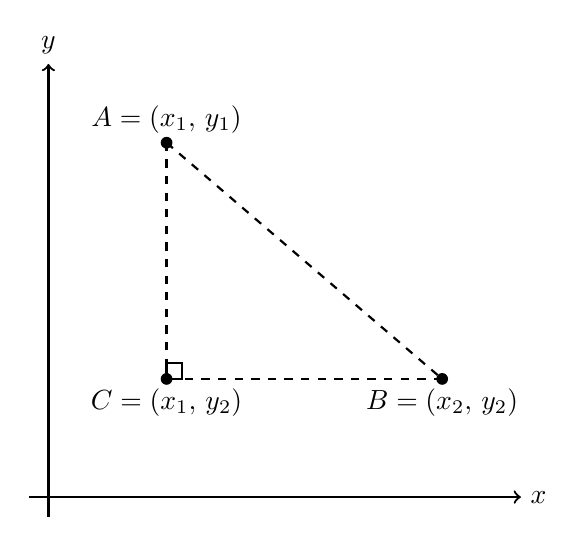
\begin{tikzpicture}[%%
  axisStyle/.style={->,thick},%%
  dashStyle/.style={-,dashed,thick},%%
  lineStyle/.style={-,thick},%%
  nodeStyle/.style={circle,inner sep=1.5pt,fill=black,black}
]
%%
%%
\pgfmathsetmacro{\dx}{0.2}
\pgfmathsetmacro{\xA}{1.5}
\pgfmathsetmacro{\xB}{5}
\pgfmathsetmacro{\xhigh}{6}
\pgfmathsetmacro{\xlow}{-0.25}
\pgfmathsetmacro{\yA}{4.5}
\pgfmathsetmacro{\yB}{1.5}
\pgfmathsetmacro{\yhigh}{5.5}
\pgfmathsetmacro{\ylow}{-0.25}
\coordinate (A) at (\xA,\yA);
\coordinate (B) at (\xB,\yB);
\coordinate (C) at (\xA,\yB);
\coordinate (xend) at (\xhigh,0);
\coordinate (xstart) at (\xlow,0);
\coordinate (yend) at (0,\yhigh);
\coordinate (ystart) at (0,\ylow);
%%
%% The Cartesian coordinate system.
\cartesianCoordinate
%%
%% A generic right-angled triangle.
%% The point A.
\xyPoint{\xA}{\yA}{A = \tuple{x_1}{y_1}}{above}
%% The point B.
\xyPoint{\xB}{\yB}{B = \tuple{x_2}{y_2}}{below}
%% The point C.
\xyPoint{\xA}{\yB}{C = \tuple{x_1}{y_2}}{below}
%% Draw the right-angled triangle as dashed lines.
\draw[dashStyle] (A) -- (B);
\draw[dashStyle] (A) -- (C);
\draw[dashStyle] (B) -- (C);
\draw[lineStyle] (C) rectangle (\xA+\dx,\yB+\dx);
\end{tikzpicture}

\end{document}
